\chapter{What is an Environment?}
\label{chap:background}

In order to see how an application's environment can contribute to the presence of bugs, it is important
to have a clear understanding
of what we mean by an environment. In this context, an environment consists of
all of the components an application depends upon
that are out of the control of their developers.
In practice, this is everything other than the code and data packaged
within the application itself.


These external elements,
illustrated in Figure~\ref{fig:environment},
can be
configured in unexpected ways.
For example, default system libraries could be loaded instead of
the versions deployed alongside the application due to the configuration of search rules for a library. 
Typically, testers
focus on explicit inputs to the application
and overlook the implicit inputs
coming from these uncontrolled components. As a result, these external resources can affect the flow of execution in unexpected ways.

An investigation of bug reports in major applications denotes several broad categories of environmental bugs. Each of these categories are discussed in greater detail below.

\begin{figure}[ht]
\centering
  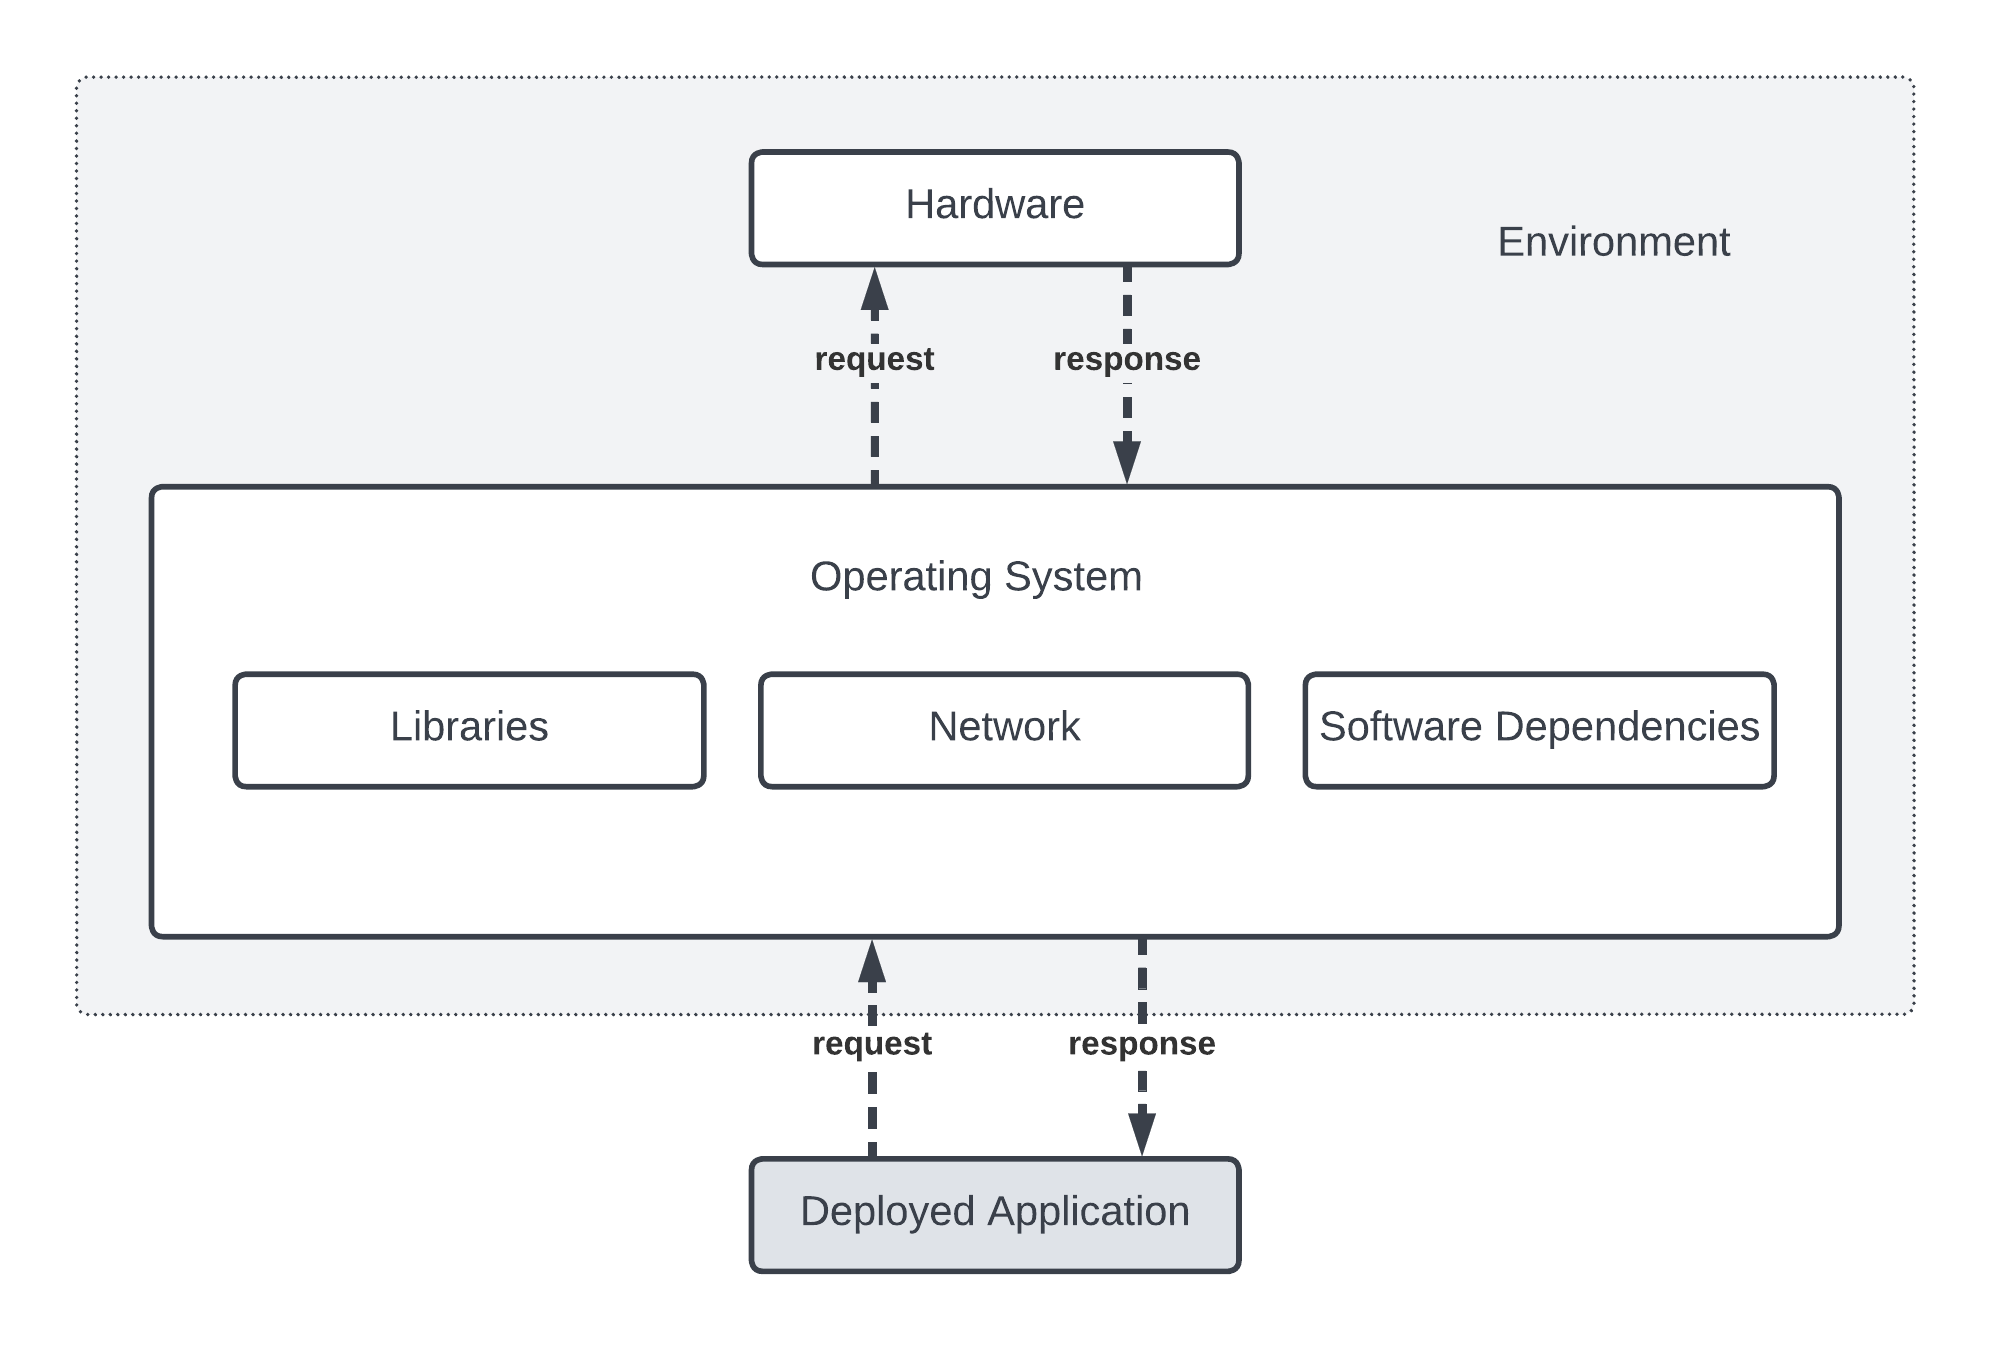
\includegraphics[frame,scale=.85]{chapter2/figures/environment}
  \caption[Overview of Environmental Influences]{
    An application's execution is influenced by a number of factors, such as the system's hardware, the
    operating system,
    and other resources.  Anomalies are often visible in the communications (represented as dashed arrows) between an application and its environment.
   }
  \label{fig:environment}
\end{figure}


\section{Operating Systems}
Applications depend upon an operating system to abstract away hardware concerns and provide services, such as network communications,
storage,
and memory management.
Options for both operating systems and operating system distributions are many, and each can differ in a number of ways. These variances could include services,
configurations,
preinstalled software,
and the executable resources provided to applications.
Though there have been numerous efforts to define standard interfaces, or develop abstractions to deal with these differences, these efforts have had only varying degrees of success.

One approach to ensuring compliant operating systems is to develop standards. In this manner, all applications would offer identically-behaving services to applications. 
Unfortunately, standards only work if they are uniformly compliant, and ensuring compliance
may take a tremendous amount of effort.
POSIX is an example of one such standard.
It defines a set of libraries, facilities, and services an operating system should provide, including test suites to prove compliance~\cite{posixoverview}.
Most of the behaviors it standardizes are present in operating systems like Linux and MacOS. But, few operating system developers have gone through the complete process of becoming ``POSIX-Certified~\cite{posixregister}.''
They instead prefer to remain ``mostly POSIX-compliant,'' which allows environmental differences to proliferate. 
For example,
POSIX-compliant regular expressions are missing features, such as back-references and commonly used shorthand characters~\cite{posixregex}.
Applications that rely on these features must identify what capabilities their environment provides and ensure they employ them properly.

Another approach has been to introduce abstraction layers, such as language virtual machines similar to those provided by Python and Java.
Such software allows developers to write applications against their own functions and APIs while relying on the chosen virtual machine to detect and handle the differences between operating systems.
For common usages this approach can work well, but there have been cases where
the abstraction is leaky.
Python's {\tt open} function, for example, may return different sorts of objects,
with differing capabilities,
depending on the underlying operating system and the file being opened~\cite{pythonopen}.

Even when operating systems provide the same functions,
there are often semantic differences between operations. 
The way operating systems
implement system calls is one such example.  In Linux, it is possible to remove an open file, yet Windows systems~\cite{UnlinkStandard} do not permit this.  If a developer writes an application
and does not keep this difference in mind, shifting from one implementation to another could lead to failure.

\section{File Systems}

The exact file system and configuration used will also have a
substantial impact on the behavior of a system, independent of the underlying
operating system. Take the popular Ext4 file system on Linux. This system is case sensitive,
so that ``a'' and ``A'' are different files.
Meanwhile, if you are using OS X's HFS+ file system,
those names would refer to the same file.
This specific difference has led to bugs in major, modern applications like Visual Studio Code~\cite{vscodebug}.

File systems can have varying limits or behaviors for other items as well. These include file name length (popularized due to the 8.3 limitations of the
FAT file system), maximum file length, number of directory entries, or
depth
of directories supported.
If these variations are not accounted for it can lead to errors~\cite{EXT4Layout, AppleHFS}.
To further complicate matters,
these limitations are independent of specific operating system limits~\cite{windowspath}.
Consider Windows,
which uses a 260 character max path limit, as compared to EXT4, which allows up to 4096 characters.
Such a conflict can lead to problems in scenarios like mixed-operating system file shares.

The layout and contents of a file system can also impact an application's
execution.  In addition, unexpected file types can result in application
failures, and multi-disk layouts may impose additional requirements on
common operations, such as moving a file from one location to
another.  We discuss this specific operation in detail in Chapter~\ref{chap:sea}.

Network-based file sharing software, such as Linux's Network File System (NFS), can add  additional opportunities for environmental differences to crop up. This type of software effectively acts as an additional file system, independent of the host file system from which it serves content.
Cases exist where applications that operate correctly on local filesystems fail when executed using shared files served from NFS~\cite{gitlabbug}.

Even the specific semantics of essential operations, such as flushing new file contents to disk can differ widely.
XFS has the ability to cache writes in memory in order to improve performance.
This means that if an application needs to ensure contents are stored on disk they must use {\tt fsync} in addition to normal calls to {\tt write}.
Failure to do so can result in data corruption should an application encounter an error before the cache is flushed~\cite{xfscorruption}.


\section{Network}
Both local and remote network nodes
can have specific characteristics that could influence the behavior of an
application.
In the simplest case,
firewalls and other traffic filtering devices can prevent necessary communications from succeeding.
In more complex cases, the network may function, but at a level insufficient for an application to work correctly.
This degraded performance can occur unintentionally due to bugs in network hardware~\cite{pfsensebug} or intentionally as part of an attempt to fairly allocate limited network resources~\cite{dlinkarticle}.
In either case, applications that depend on a stable network connection can fail.

Even if a network performs well,
the specific details of how an operating system handles network communications can introduce problems.
For example, POSIX operating
systems support the notion of limiting the kernel buffer set aside for a
socket.  However, many other popular operating
systems such as (Windows, Linux, and Mac)
implement this quite differently.
If a UDP datagram
larger than the specified buffer size is received by a Linux system,
it will be dropped.
Windows,
however,
will receive these datagrams,
but
any system calls that retrieve data from the buffer
will only return a number of bytes less than or equal to the
buffer size, requiring multiple calls
to retrieve all the data.~\cite{Zhuang_NSDI_2014}.

\section{Processor}
Lastly, the processor used can also influence the
behavior of an application.  This is frequently
evidenced through the different floating point behaviors a
processor may exhibit~\cite{ArbitraryPrecision}.
In addition, bugs are fairly common
in processors and will cause variances, as will
differences in interpreting
how to execute complex instructions~\cite{Microarch}.

This problem is exacerbated by the increasing variety of processors, both hardware and virtualized, in use in real world scenarios.
After a period of dominance,
x86-based processors are being replaced with ARM-based alternatives in some scenarios.
A major shift occurred when Apple began shipping laptops that use their own ARM-based M1 processor.
As developers began using these laptops,
subtle portability issues resulting from hardware differences appeared.
The impacts of these issues include massive performance hits~\cite{ghccompile}, 

Virtualized hardware has similar concerns.
In some cases emulated hardware handles important instructions differently than its physical counterpart~\cite{unicornbug}.
Occasionally,
such hardware will completely omit features that some applications require in order to work correctly.
We encountered this issue when working with the {\tt rr}
record-and-replay debugger under various pieces of virtualization software.
{\tt rr} uses hardware performance counters to correctly replicate thread interleaving during replay. Yet,
at the time of this writing,
only VMWare products supported virtualized hardware performance counters~\cite{vmwarecounters}.
While {\tt rr} is able to detect and report the absence of this capability,
this case illustrates why it's important to  know the environment before deploying an application.

% spectre apps run slower after fixes 



